% !TEX root = ./Basilisk-celestialTwoBodyPoint-20190311.tex

\section{Model Description}


\subsection{Module Goal}
This module computes a reference whose aim is to track the center of a primary target, e.g. pointing the communication antenna at the Earth, at the same time of trying to meet a secondary constraint as best as possible, e.g. a solar panel normal axis pointing the closest in the direction of the Sun.  It is important to note that two pointing conditions in a three-dimensional space compose an overdetermined problem. Thus, the main constraint is always priorized over the secondary one so the former can always be met.\\
Figure~\ref{fig:fig1} shows the case where Mars is the primary celestial body and the Sun is the secondary one. Note that the origin of the desired reference frame $\mathcal{R}$ is the position of the spacecraft.
\begin{figure}[htb]
	\centerline{
	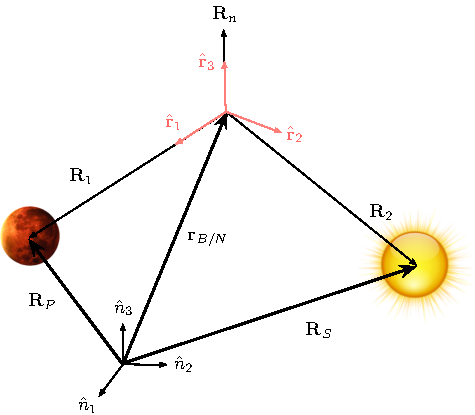
\includegraphics[]{Figures/fig1.pdf}
	}
	\caption{Illustration of the restricted two-body pointing reference frame $\mathcal{R}:\{ \hat{\bm r}_{1},\hat{\bm r}_{1}, \hat{\bm r}_{2} \}$ and the inertial frame $\mathcal{N}:\{ \hat{\bm n}_{1},\hat{\bm n}_{1}, \hat{\bm n}_{2} \}$.}
	\label{fig:fig1}
\end{figure}

Assuming knowledge of the position of the spacecraft $\bm{r}_{B/N}$ and the involved celestial bodies, $\bm{R}_{P1}$ and  $\bm{R}_{P2}$ (all of them relative to the inertial frame $\mathcal{N}$ and expressed in inertial frame components), the relative position of the celestial bodies with respect to the spacecraft is obtained by simple subtraction:
\begin{subequations}
	\begin{align}
		 \bm{R}_{P1} =\bm{R}_{P} - \bm{r}_{B/N} \\
		 \bm{R}_{P2} =\bm{R}_{S} - \bm{r}_{B/N}
	\end{align}
\end{subequations}

In analogy, the inertial derivatives of these position vectors are obtained:
\begin{subequations}
	\begin{align}
		 \bm{v}_{P1} &=\bm{v}_{P} - \bm{v}_{B/N} \\
		 \bm{v}_{P2} &=\bm{v}_{S} - \bm{v}_{B/N} \\
		 \bm{a}_{P1} &=\bm{a}_{P} - \bm{a}_{B/N} \\
		 \bm{a}_{P2} &=\bm{a}_{S} - \bm{a}_{B/N}
	\end{align}
\end{subequations}

The normal vector $\bm{R}_{n}$ of the plane defined by $\bm{R}_{P1}$ and $\bm{R}_{P2}$ is computed through:
\begin{equation}
	\bm R_{n} =\bm{R}_{P1} \times \bm{R}_{P2}
\end{equation}
The inertial time derivative of $\bm{R}_n$ is found using the chain differentiation rule:
\begin{equation}
	\bm {v}_{n} = \bm{v}_{P1} \times \bm{R}_{P2} + \bm{R}_{P1} \times \bm{v}_{P2}
\end{equation}
And the second time derivative:
\begin{equation}
	\bm {a}_{n} = \bm{a}_{P1} \times \bm{R}_{P2} + \bm{R}_{P1} \times \bm{a}_{P2}  + 2 \bm{v}_{P1} \times \bm{v}_{P2}
\end{equation}
\subsection{ Special Case: No Secondary Constraint Applicable}
If there is no incoming message with a secondary celestial body pointing condition or if the constrain is not valid, an artificial three-dimensional frame is defined instead. Note that a single condition pointing leaves one degree of freedom, hence standing for an underdetermined attitude problem. A secondary constrain is considered to be invalid if the angle between $\bm{R}_{P1}$ and $\bm{R}_{P2}$ is, in absolute value, minor than a set threshold. This could be the case where the primary and secondary celestial bodies are aligned as seen by the spacecraft. In such situation, the primary pointing axis would already satisfy both the primary and the secondary constraints.

Since the main algorithm of this module, which is developed in the following sections, assumes two conditions, the second one is arbitrarily set as following:
\begin{equation}
	\bm{R}_{P2} = \bm{R}_{P1} \times \bm{v}_{P1} \equiv  \bm{h}_{P1}
\end{equation}
By setting the secondary constrain to have the direction of the angular momentum vector $ \bm{h}_{P1}$, it is assured that it will always be valid ($\bm{R}_{P1}$ and $\bm{R}_{P2}$ are now perpendicular).
The first and second time derivatives are steadily computed:
\begin{equation}
	\bm{v}_{P2} =  \bm{R}_{P1} \times \bm{a}_{P1}
\end{equation}
\begin{equation}
	\bm{a}_{P2} =  \bm{v}_{P1} \times \bm{a}_{P1}
\end{equation}
\subsection{Reference Frame Definition}
As illustrated in Figure~\ref{fig:fig1}, the base vectors of the desired reference frame $\mathcal{R}$  are defined as following:
\begin{subequations}
	\begin{align}
		\hat{\bm r}_{1} &= \frac{{\bm R}_{P1}} {|{\bm R}_{P1}|} \\
		\hat{\bm r}_{3} &= \frac{{\bm R}_{n}}{|{\bm R}_{n}|} \\
		\hat{\bm r}_{2} &=  \hat{\bm r}_{3} \times \hat{\bm r}_{1}
	\end{align}
\end{subequations}
Since the position vectors are given in terms of inertial $\mathcal{N}$-frame components, the DCM from the inertial frame $\mathcal{N}$ to the desired reference frame $\mathcal{R}$ is:
\begin{equation}
	[RN] = \begin{bmatrix}
		\leftexp{N}{ \hat{\bm r}_{1}^{T} } \\
		\leftexp{N}{ \hat{\bm r}_{2}^{T} }  \\
		\leftexp{N}{ \hat{\bm r}_{3}^{T} }
	\end{bmatrix}
\end{equation}
\subsection{Base Vectors Time Derivatives}
Dots denote inertial time derivatives. In the matrix expressions below, all vectors and their derivatives are expressed in inertial $\mathcal{N}$-frame components. Thus, the arrays \texttt{r1\_hat\_N}, \texttt{dr1\_hat\_N}, and \texttt{ddr1\_hat\_N} represent a basis vector and its first two inertial derivatives, all in the same component frame.

Define the projection matrices
\[
    C_i = I_{3\times3} - \hat{\bm r}_i\hat{\bm r}_i^T,
    \qquad i\in\{1,3\}.
\]
These are projections orthogonal to the indicated basis vector, not direction cosine matrices. The first derivatives are
\begin{subequations}
    \begin{align}
        \dot{\hat{\bm r}}_1 &= C_1 \frac{\bm v_{P1}}{|\bm R_{P1}|}, \\
        \dot{\hat{\bm r}}_3 &= C_3 \frac{\bm v_n}{|\bm R_n|}, \\
        \dot{\hat{\bm r}}_2 &= \dot{\hat{\bm r}}_3 \times \hat{\bm r}_1
                              + \hat{\bm r}_3 \times \dot{\hat{\bm r}}_1.
    \end{align}
\end{subequations}
For example, differentiating the normalized primary direction gives
\begin{subequations}
    \begin{align}
        \dot{\hat{\bm r}}_1
            &= \frac{d}{dt}\left(\frac{\bm R_{P1}}{|\bm R_{P1}|}\right), \\
            &= \frac{\bm v_{P1}}{|\bm R_{P1}|}
               - \frac{\bm R_{P1}(\bm R_{P1}\cdot\bm v_{P1})}{|\bm R_{P1}|^3}, \\
            &= \frac{1}{|\bm R_{P1}|}
               (I_{3\times3}-\hat{\bm r}_1\hat{\bm r}_1^T)\bm v_{P1}.
    \end{align}
\end{subequations}
The second derivatives are
\begin{subequations}
    \begin{align}
        \ddot{\hat{\bm r}}_1
            &= \frac{C_1\bm a_{P1}
               -(2\dot{\hat{\bm r}}_1\hat{\bm r}_1^T
                  +\hat{\bm r}_1\dot{\hat{\bm r}}_1^T)\bm v_{P1}}
               {|\bm R_{P1}|}, \\
        \ddot{\hat{\bm r}}_3
            &= \frac{C_3\bm a_n
               -(2\dot{\hat{\bm r}}_3\hat{\bm r}_3^T
                  +\hat{\bm r}_3\dot{\hat{\bm r}}_3^T)\bm v_n}
               {|\bm R_n|}, \\
        \ddot{\hat{\bm r}}_2
            &= \ddot{\hat{\bm r}}_3\times\hat{\bm r}_1
               +\hat{\bm r}_3\times\ddot{\hat{\bm r}}_1
               +2\dot{\hat{\bm r}}_3\times\dot{\hat{\bm r}}_1.
    \end{align}
\end{subequations}
In particular, the two outer-product terms inside each parenthesis have the same sign. This follows from
\begin{subequations}
    \begin{align}
        \dot C_1 &= -\dot{\hat{\bm r}}_1\hat{\bm r}_1^T
                    -\hat{\bm r}_1\dot{\hat{\bm r}}_1^T, \\
        \frac{d}{dt}|\bm R_{P1}| &= \hat{\bm r}_1\cdot\bm v_{P1}, \\
        \ddot{\hat{\bm r}}_1
            &= \frac{C_1\bm a_{P1}+\dot C_1\bm v_{P1}
                -\dot{\hat{\bm r}}_1(\hat{\bm r}_1\cdot\bm v_{P1})}
                {|\bm R_{P1}|}.
    \end{align}
\end{subequations}

\subsection{Angular Velocity and Acceleration Descriptions}
The angular velocity projections onto the reference basis satisfy
\begin{subequations}
    \begin{align}
        \bm\omega_{R/N}\cdot\hat{\bm r}_1 &= \hat{\bm r}_3\cdot\dot{\hat{\bm r}}_2, \\
        \bm\omega_{R/N}\cdot\hat{\bm r}_2 &= \hat{\bm r}_1\cdot\dot{\hat{\bm r}}_3, \\
        \bm\omega_{R/N}\cdot\hat{\bm r}_3 &= \hat{\bm r}_2\cdot\dot{\hat{\bm r}}_1.
    \end{align}
\end{subequations}
Differentiating the left-hand sides introduces the terms
$\bm\omega_{R/N}\cdot\dot{\hat{\bm r}}_i$. Each term is zero because the basis rotates with the reference frame:
\[
    \dot{\hat{\bm r}}_i=\bm\omega_{R/N}\times\hat{\bm r}_i,
    \qquad
    \bm\omega_{R/N}\cdot\dot{\hat{\bm r}}_i=0.
\]
Consequently, the angular acceleration projections are
\begin{subequations}
    \begin{align}
        \dot{\bm\omega}_{R/N}\cdot\hat{\bm r}_1
            &= \dot{\hat{\bm r}}_3\cdot\dot{\hat{\bm r}}_2
               +\hat{\bm r}_3\cdot\ddot{\hat{\bm r}}_2, \\
        \dot{\bm\omega}_{R/N}\cdot\hat{\bm r}_2
            &= \dot{\hat{\bm r}}_1\cdot\dot{\hat{\bm r}}_3
               +\hat{\bm r}_1\cdot\ddot{\hat{\bm r}}_3, \\
        \dot{\bm\omega}_{R/N}\cdot\hat{\bm r}_3
            &= \dot{\hat{\bm r}}_2\cdot\dot{\hat{\bm r}}_1
               +\hat{\bm r}_2\cdot\ddot{\hat{\bm r}}_1.
    \end{align}
\end{subequations}
These scalar projections are the R-frame components, although the implementation evaluates each dot product using basis vectors and derivatives in N-frame components:
\begin{equation}
    \leftexp{R}{\bm\omega_{R/N}} =
    \begin{bmatrix}
        \bm\omega_{R/N}\cdot\hat{\bm r}_1 \\
        \bm\omega_{R/N}\cdot\hat{\bm r}_2 \\
        \bm\omega_{R/N}\cdot\hat{\bm r}_3
    \end{bmatrix}.
\end{equation}
Similarly,
\begin{equation}
    \leftexp{R}{\dot{\bm\omega}_{R/N}} =
    \begin{bmatrix}
        \dot{\bm\omega}_{R/N}\cdot\hat{\bm r}_1 \\
        \dot{\bm\omega}_{R/N}\cdot\hat{\bm r}_2 \\
        \dot{\bm\omega}_{R/N}\cdot\hat{\bm r}_3
    \end{bmatrix}.
\end{equation}
Dotting \texttt{omega\_RN\_R} with \texttt{dr1\_hat\_N}, or either of the other basis derivatives, mixes component frames and does not evaluate the zero-valued geometric term. The implementation omits these terms.

Finally, the output message contains N-frame components. Since $[RN]$ maps N to R, the inverse transformation is $[NR]=[RN]^T$:
\begin{subequations}
    \begin{align}
        \leftexp{N}{\bm\omega_{R/N}} &= [RN]^T\,\leftexp{R}{\bm\omega_{R/N}}, \\
        \leftexp{N}{\dot{\bm\omega}_{R/N}} &= [RN]^T\,\leftexp{R}{\dot{\bm\omega}_{R/N}}.
    \end{align}
\end{subequations}
